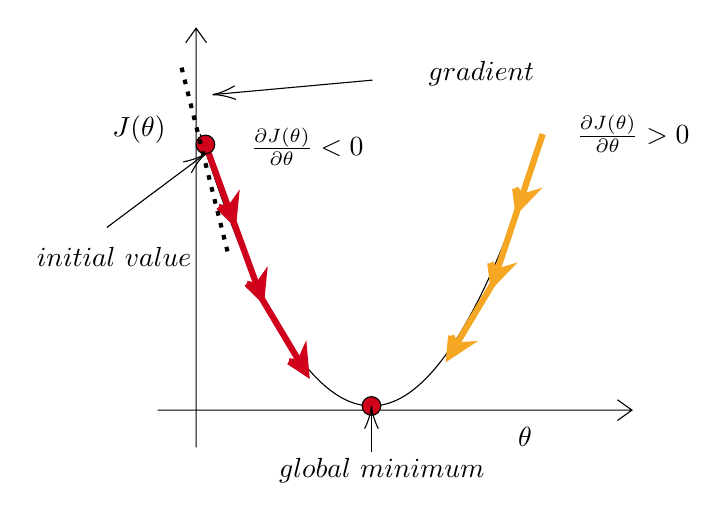
\begin{tikzpicture}[x=0.75pt,y=0.75pt,yscale=-1,xscale=1]
%uncomment if require: \path (0,300); %set diagram left start at 0, and has height of 300

\draw  (75,190) -- (303.5,190)(93.5,6) -- (93.5,208) (296.5,185) -- (303.5,190) -- (296.5,195) (88.5,13) -- (93.5,6) -- (98.5,13)  ;
\draw   (95.5,57) .. controls (150.5,231.67) and (205.5,231.67) .. (260.5,57) ;
\draw [color={rgb, 255:red, 208; green, 2; blue, 27 }  ,draw opacity=1 ][line width=2.25]    (98,62) -- (111.5,99) ;
\draw [shift={(111.5,99)}, rotate = 249.95] [color={rgb, 255:red, 208; green, 2; blue, 27 }  ,draw opacity=1 ][fill={rgb, 255:red, 208; green, 2; blue, 27 }  ,fill opacity=1 ][line width=2.25]   (8.93,-4.29) -- (0,0) -- (8.93,4.29) -- (5.93,0) -- (8.93,-4.29)    ;

\draw [color={rgb, 255:red, 208; green, 2; blue, 27 }  ,draw opacity=1 ][line width=2.25]    (111.5,99) -- (125,136) ;
\draw [shift={(125,136)}, rotate = 249.95] [color={rgb, 255:red, 208; green, 2; blue, 27 }  ,draw opacity=1 ][fill={rgb, 255:red, 208; green, 2; blue, 27 }  ,fill opacity=1 ][line width=2.25]   (8.93,-4.29) -- (0,0) -- (8.93,4.29) -- (5.93,0) -- (8.93,-4.29)    ;

\draw [color={rgb, 255:red, 208; green, 2; blue, 27 }  ,draw opacity=1 ][line width=2.25]    (125,136) -- (146.5,172) ;
\draw [shift={(146.5,172)}, rotate = 239.15] [color={rgb, 255:red, 208; green, 2; blue, 27 }  ,draw opacity=1 ][fill={rgb, 255:red, 208; green, 2; blue, 27 }  ,fill opacity=1 ][line width=2.25]   (8.93,-4.29) -- (0,0) -- (8.93,4.29) -- (5.93,0) -- (8.93,-4.29)    ;

\draw [color={rgb, 255:red, 245; green, 166; blue, 35 }  ,draw opacity=1 ][line width=2.25]    (260.5,57) -- (248.5,93) ;
\draw [shift={(248.5,93)}, rotate = 288.43] [color={rgb, 255:red, 245; green, 166; blue, 35 }  ,draw opacity=1 ][fill={rgb, 255:red, 245; green, 166; blue, 35 }  ,fill opacity=1 ][line width=2.25]   (8.93,-4.29) -- (0,0) -- (8.93,4.29) -- (5.93,0) -- (8.93,-4.29)    ;

\draw [color={rgb, 255:red, 245; green, 166; blue, 35 }  ,draw opacity=1 ][line width=2.25]    (248.5,93) -- (236.5,129) ;
\draw [shift={(236.5,129)}, rotate = 288.43] [color={rgb, 255:red, 245; green, 166; blue, 35 }  ,draw opacity=1 ][fill={rgb, 255:red, 245; green, 166; blue, 35 }  ,fill opacity=1 ][line width=2.25]   (8.93,-4.29) -- (0,0) -- (8.93,4.29) -- (5.93,0) -- (8.93,-4.29)    ;

\draw [color={rgb, 255:red, 245; green, 166; blue, 35 }  ,draw opacity=1 ][line width=2.25]    (236.5,129) -- (215.5,164) ;
\draw [shift={(215.5,164)}, rotate = 300.96] [color={rgb, 255:red, 245; green, 166; blue, 35 }  ,draw opacity=1 ][fill={rgb, 255:red, 245; green, 166; blue, 35 }  ,fill opacity=1 ][line width=2.25]   (8.93,-4.29) -- (0,0) -- (8.93,4.29) -- (5.93,0) -- (8.93,-4.29)    ;

\draw  [fill={rgb, 255:red, 208; green, 2; blue, 27 }  ,fill opacity=1 ]  (98, 62) circle [x radius= 4.5, y radius= 4.5]  ;
\draw    (50.5,102) -- (98,66.5) ;
\draw [shift={(98,66.5)}, rotate = 503.23] [color={rgb, 255:red, 0; green, 0; blue, 0 }  ]   (0,0) .. controls (3.31,-0.3) and (6.95,-1.4) .. (10.93,-3.29)(0,0) .. controls (3.31,0.3) and (6.95,1.4) .. (10.93,3.29)   ;

\draw  [fill={rgb, 255:red, 208; green, 2; blue, 27 }  ,fill opacity=1 ]  (178, 188) circle [x radius= 4.5, y radius= 4.5]  ;
\draw    (178,210) -- (178,188) ;
\draw [shift={(178,188)}, rotate = 450] [color={rgb, 255:red, 0; green, 0; blue, 0 }  ]   (0,0) .. controls (3.31,-0.3) and (6.95,-1.4) .. (10.93,-3.29)(0,0) .. controls (3.31,0.3) and (6.95,1.4) .. (10.93,3.29)   ;

\draw [line width=1.5]  [dash pattern={on 1.69pt off 2.76pt}]  (86.5,25) -- (109.5,117) ;


\draw    (178.5,31) -- (101.5,38) ;
\draw [shift={(101.5,38)}, rotate = 354.81] [color={rgb, 255:red, 0; green, 0; blue, 0 }  ]   (0,0) .. controls (3.31,-0.3) and (6.95,-1.4) .. (10.93,-3.29)(0,0) .. controls (3.31,0.3) and (6.95,1.4) .. (10.93,3.29)   ;


\draw (252,203) node   {$\theta$};
\draw (66,55) node   {$J( \theta)$};
\draw (147,63) node   {$\frac{\partial J(\theta)}{\partial \theta} < 0$};
\draw (304,57) node   {$\frac{\partial J(\theta)}{\partial \theta}  >0$};
\draw (183,219) node   {$global\ minimum$};
\draw (54,116) node   {$initial\ value$};
\draw (231,28) node   {$gradient$};


\end{tikzpicture}
